\documentclass[12pt]{article}
\usepackage[hmargin=2.0cm,vmargin=1cm]{geometry}
\usepackage[utf8]{inputenc}
\usepackage{graphicx}
\usepackage{float}
\usepackage{cite}
\usepackage{natbib}
\usepackage{amsmath}

\title{\begin{LARGE}
{$\Delta_{vir}$}
\end{LARGE}}

\begin{document}
\maketitle


\section{Useful Quantities and definitions}

In this section some common quantities useful for describe the denstites profile
are defined and explained. 


\subsection{Critical density of the Universe:}

\subsection{Virialization}

A dark matter halo is virialized when its in equilibrium, such 
an equilibrium occurs after the dark matter have collapsed and 
the force of gravity equals the \textbf{relaxtion} processes
(Binney \& Tremaine pag 380).


\textbf{How is related the virialization with the radius, since what redshift 
you can define a $r_{vir}$}

A halo can be characterized using and overdensity $\Delta{vir}$
defined as ratio of the density of a virialized halo over the critical 
density of the Universe $\Delta_{vir} = \frac{\rho_{vir}}{\rho_c}$.
For a cosmolgy with ($\Omega_m + \Omega_{\Lambda} = 1$) 
\begin{equation}
\Delta_{vir} = (18 \pi^2 + 82x - 39x^2)/\Omega(z) 
\end{equation}
(Bryan \& Norman 1998) it's a good approximation, here $x=\Omega(z)-1$.
For the present time ($z=0$)  $\Delta_{vir}=360$.

\verb+http://arxiv.org/pdf/astro-ph/9710107v1.pdf+ \\
\verb+http://arxiv.org/pdf/astro-ph/9601088v1.pdf+


\begin{figure}[h]
\centering
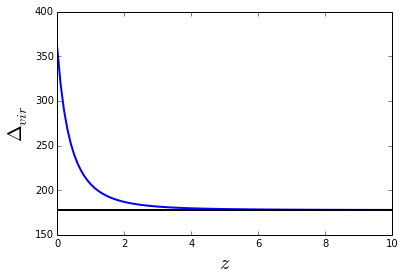
\includegraphics[scale=0.7]{deltavir.png}
\end{figure}


This overdensity is enclosed in a volume which can be charcterized
with a radius $r_{vir}$ which correspond to a $M_{vir}$ given 
$\Delta_{rvir}$

\begin{equation}
\rho_{vir} = \frac{3M_{vir}}{4 \pi r_{vir}^3} = \Delta_{vir} \Omega_m \rho_{crit} 
\end{equation}

\begin{equation}
r_{vir} = \left( \frac{3M_{vir}}{4 \pi \Delta_{vir} \Omega_m \rho_{crit} } \right )^{1/3}
\end{equation}

For example for a halo of mass $M = 1 \times 10^{12}M_{\odot}$ the corresponding radius is $r_{vir}=262.4$ Kpc

\subsection{$r_{200}$ \& $M_{200}$}

\begin{equation}
M_{200} = 200 \rho_c \dfrac{4}{3} \pi r_{200}^3
\end{equation}

\begin{equation}
M_{vir} = \Delta_{vir} \Omega_m \rho_c \dfrac{4}{3} \pi r_{vir}^3
\end{equation}


Matching $rho_c$ for the above two equations we get.

\begin{equation}
\dfrac{M_{200}}{M_{vir}} = \left(  \dfrac{200}{ \Delta_{vir} \Omega_m}  \right) \left( \dfrac{r_{200}}{r_{vir}}  \right)^3
\end{equation}

Here is common to call $q = \left(  \dfrac{200}{ \Delta_{vir} \Omega_m}  \right) $ at $z=0$ $q=2.053$ 

\begin{equation}
\dfrac{M_{200}}{M_{vir}} = q \left( \dfrac{r_{200}}{r_{vir}}  \right)^3
\end{equation} 
 

\section{Densities profiles}

\subsection{Plummer}

The plumer density profile is one of the simplest models which describes
a constant density near the center and falls at large radius.

\begin{equation}
\rho_P (r) = \frac{3M}{4\pi a^3} (1 + \frac{r^2}{a^2})^{-5/2}
\end{equation} 

Where $a$ is call the scale length. The scale length set the length $a$ in which the mayority of the density is enclosed. Note
that if $a$ is cero the plummer potential would be exactly as the potential of a point mass. 
In the other hand if $a$ goes to infty the potential is rewpresenting a very extended mass source.
In other words the scale length set up the size of the volume in which the mass $M$ is enclosed.

The enclosed mass can be derived from the density by integrating over a volume. 

\begin{equation}
M_P(<r) = 4 \pi \int_0^r r'^2\frac{3M}{4\pi a^3} (1 + \frac{r'^2}{a^2})^{-5/2} dr' = \frac{3M}{a^3} \left( \frac{a^4 r^3 \sqrt{r^2/a^2 + 1}}{3(r^2 + a^2)^2}  \right)
\end{equation}

\begin{equation}
M_P(<r) = M \frac{r^3}{(a^2+r^2)^{3/2}}
\end{equation}


\subsection{Hernquist}


\subsection{Isothermal}

\subsection{NFW}


\end{document}
